\documentclass[11pt,a4paper]{scrartcl}

% ============================================
% Pakete
% ============================================
\usepackage[utf8]{inputenc}
\usepackage[T1]{fontenc}
\usepackage[ngerman]{babel}
\usepackage{amsmath,amssymb}
\usepackage{siunitx}
\sisetup{locale=DE, per-mode=fraction}
\usepackage{graphicx}
\usepackage{booktabs}
\usepackage{array}
\usepackage{tcolorbox}
\tcbuselibrary{skins, breakable}
\usepackage{fontawesome5}
\usepackage{tikz}
\usetikzlibrary{shapes.geometric, arrows.meta, positioning, decorations.pathmorphing}
\usepackage{scrlayer-scrpage}
\usepackage{geometry}
\geometry{left=2cm, right=2cm, top=2.5cm, bottom=2cm, headheight=1.5cm}

% ============================================
% Kopf- und Fußzeile (KOMA-Script)
% ============================================
\clearpairofpagestyles
\ihead{
\includegraphics[height=1cm]{logo.jpeg}}
\chead{\textbf{Physik-LK 11NP}}
\ohead{\textbf{\today}}
\cfoot{\pagemark}
\KOMAoptions{headsepline=0.4pt}

% ============================================
% tcolorbox-Definitionen
% ============================================
\newtcolorbox{formelbox}[1][]{
	colback=blue!5!white,
	colframe=blue!75!black,
	fonttitle=\bfseries,
	title={\faIcon{square-root-alt} Formel},
	#1
}

\newtcolorbox{aufgabe}[1][]{
	colback=orange!5!white,
	colframe=orange!75!black,
	fonttitle=\bfseries,
	title={\faIcon{pencil-alt} Aufgabe},
	#1
}

\newtcolorbox{hilfebox}[1][]{
	colback=green!5!white,
	colframe=green!60!black,
	fonttitle=\bfseries,
	title={\faIcon{lightbulb} Hinweis},
	#1
}

\newtcolorbox{infobox}[1][]{
	colback=gray!5!white,
	colframe=gray!75!black,
	fonttitle=\bfseries,
	title={\faIcon{info-circle} Information},
	#1
}

\newtcolorbox{materialbox}[1][]{
	colback=purple!5!white,
	colframe=purple!75!black,
	fonttitle=\bfseries,
	title={\faIcon{tools} Materialien},
	#1
}

\setlength{\parindent}{0pt}
\setlength{\parskip}{0.4em}

% ============================================
% Dokumentbeginn
% ============================================
\begin{document}
	
	% ============================================
	% Titel
	% ============================================
	\begin{center}
		{\LARGE\bfseries Experiment 2: Bewegung mit konstanter Beschleunigung}\\[0.3cm]
		{\large Gleichmäßig beschleunigte Bewegung}
	\end{center}
	
	\vspace{0.3cm}
	
	% ============================================
	% Theoretischer Hintergrund
	% ============================================
	\section*{Theoretischer Hintergrund}
	
	Ändert ein Körper seine Geschwindigkeit, so spricht man von einer \textbf{beschleunigten Bewegung}. Nimmt die Geschwindigkeit gleichmäßig zu, legt der Körper in gleichen Zeiten immer größere Wege zurück.
	
	\begin{formelbox}[title={\faIcon{square-root-alt} Beschleunigung und Bewegungsgleichungen}]
		\textbf{Beschleunigung} (Geschwindigkeitsänderung pro Zeit):
		\[a = \frac{\Delta v}{\Delta t} = \frac{v_2 - v_1}{t_2 - t_1} \qquad \text{mit } v_1 = 0, t_1 = 0: \quad a = \frac{v}{t}\]
		
		\textbf{Einheit:} $[a] = \SI{1}{\metre\per\second\squared}$
		
		\vspace{0.3cm}
		\textbf{Geschwindigkeit-Zeit-Gesetz:} \quad $v = a \cdot t$
		
		\textbf{Weg-Zeit-Gesetz:} \quad $s = \frac{1}{2} \cdot a \cdot t^2$
	\end{formelbox}
	
	\vspace{0.2cm}
	
	\begin{center}
		\begin{tikzpicture}[scale=0.85]
			% t-v-Diagramm
			\begin{scope}[xshift=0cm]
				\draw[->] (0,0) -- (4.5,0) node[right] {$t$ in s};
				\draw[->] (0,0) -- (0,3.5) node[above] {$v$ in $\frac{\text{m}}{\text{s}}$};
				\draw[thick, red] (0,0) -- (4,3);
				\fill[red!30, opacity=0.5] (0,0) -- (3,0) -- (3,2.25) -- cycle;
				\draw[dashed] (3,0) node[below] {$t$} -- (3,2.25) -- (0,2.25) node[left] {$v$};
				\node at (1.5,0.6) {$s = \frac{1}{2} v \cdot t$};
				\node[below] at (2,-0.8) {\textbf{$t$-$v$-Diagramm}};
				\node[right] at (4,3) {\small Steigung $= a$};
			\end{scope}
			
			% t-s-Diagramm
			\begin{scope}[xshift=7cm]
				\draw[->] (0,0) -- (4.5,0) node[right] {$t$ in s};
				\draw[->] (0,0) -- (0,3.5) node[above] {$s$ in m};
				\draw[thick, blue, domain=0:3.5, samples=50] plot (\x, {0.25*\x*\x});
				\node[below] at (2,-0.8) {\textbf{$t$-$s$-Diagramm}};
				\node[right, blue] at (3.5,3) {\small Parabel};
			\end{scope}
		\end{tikzpicture}
	\end{center}
	
	\begin{hilfebox}
		Im $t$-$v$-Diagramm ergibt sich eine \textbf{Gerade durch den Ursprung} mit Steigung $a$.\\
		Im $t$-$s$-Diagramm ergibt sich eine \textbf{Parabel}. Trägt man $s$ über $t^2$ auf, erhält man eine Gerade mit Steigung $\frac{a}{2}$.
	\end{hilfebox}
	
	% ============================================
	% Versuchsaufbau
	% ============================================
	\section*{Versuchsaufbau}
	
	\begin{materialbox}
		\begin{minipage}{0.48\textwidth}
			\begin{itemize}
				\item Fahrbahn mit Wagen
				\item Umlenkrolle
				\item Zeit-Registriergerät
			\end{itemize}
		\end{minipage}
		\begin{minipage}{0.48\textwidth}
			\begin{itemize}
				\item Gewicht \SI{10,2}{\gram} (Antrieb)
				\item Gewicht \SI{100}{\gram} (Zusatzmasse)
				\item Registrierstreifen
			\end{itemize}
		\end{minipage}
	\end{materialbox}
	
	\vspace{0.3cm}
	
	\begin{figure}[h]
		\centering
		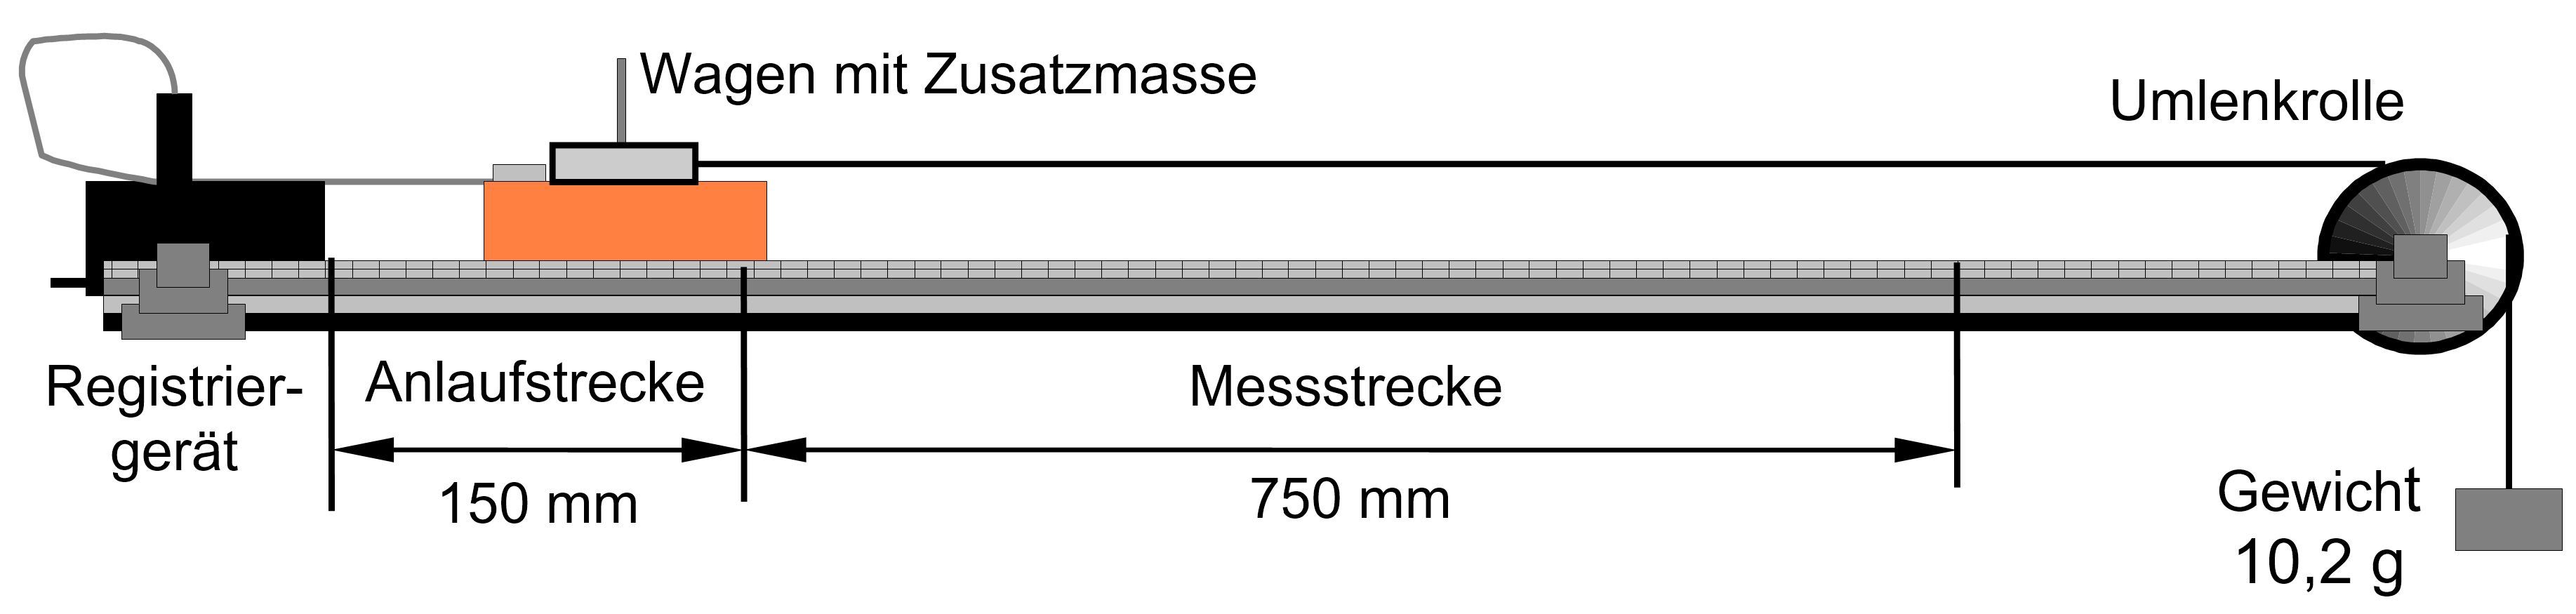
\includegraphics[width=0.95\textwidth]{fahrbahn.png}
		\caption{Versuchsaufbau mit Fahrbahn, Zeit-Registriergerät und Antriebsmasse}
		\label{fig:fahrbahn2}
	\end{figure}
	
	% ============================================
	% Durchführung
	% ============================================
	\section*{Durchführung}
	
	Bauen Sie den Versuch gemäß Abbildung~\ref{fig:fahrbahn2} auf.
	
	\begin{enumerate}
		\item Bauen Sie die Fahrbahn mit Zeit-Registriergerät und Umlenkrolle auf.
		\item Bestücken Sie den Wagen mit der Zusatzmasse (\SI{100}{\gram}).
		\item Kompensieren Sie die Reibung durch leichte Neigung der Fahrbahn.
		\item Stellen Sie das Registriergerät auf \textbf{10 Hz} ein.
		\item Das Gewicht treibt den Wagen \textbf{über die gesamte Messstrecke} an.
		\item Führen Sie die Messung durch und beschriften Sie den Streifen.
	\end{enumerate}
	
	\begin{hilfebox}[title={\faIcon{lightbulb} Unterschied zu Experiment 1}]
		Anders als bei der gleichförmigen Bewegung wirkt die Antriebskraft hier \textbf{während der gesamten Messung}. Der Wagen wird kontinuierlich beschleunigt!
	\end{hilfebox}
	
	% ============================================
	% Aufgaben
	% ============================================
	\section*{Aufgabenstellungen}
	
	\begin{aufgabe}[title={\faIcon{pencil-alt} Aufgaben}]
		\begin{enumerate}
			\item Nehmen Sie einen Registrierstreifen mit \textbf{10 Hz}-Einstellung auf.
			\item Tragen Sie die Messwerte für $s$ und $t$ in die Tabelle ein.
			\item Zeichnen Sie das $t$-$s$-Diagramm.
			\item Berechnen Sie die Intervallgeschwindigkeiten $v$ und tragen Sie diese ein.
			\item Zeichnen Sie das $t$-$v$-Diagramm.
			\item Bestimmen Sie die Beschleunigung $a$ aus der Steigung im $t$-$v$-Diagramm.
		\end{enumerate}
	\end{aufgabe}
	
	% ============================================
	% Protokollbogen
	% ============================================
	\newpage
	\section*{Protokollbogen -- Experiment 2}
	
	\begin{center}
		\begin{tcolorbox}[colback=white, colframe=black, width=\textwidth, boxrule=0.5pt]
			\begin{tabular}{@{}p{0.32\textwidth}p{0.32\textwidth}p{0.32\textwidth}@{}}
				\textbf{Name:} \hrulefill & \textbf{Klasse:} \hrulefill & \textbf{Datum:} \hrulefill \\[0.4cm]
				\textbf{Gruppenmitglieder:} & \multicolumn{2}{l}{\hrulefill} \\
			\end{tabular}
		\end{tcolorbox}
	\end{center}
	
	\subsection*{1. Messwerte (aus dem Registrierstreifen ablesen)}
	
	\begin{center}
		\renewcommand{\arraystretch}{1.8}
		\begin{tabular}{|c|c|c|c|c|c|c|c|c|}
			\hline
			$t$ in s & 0 & 0,1 & 0,2 & 0,3 & 0,4 & 0,5 & 0,6 & 0,7 \\
			\hline
			$s$ in mm & 0 & & & & & & & \\
			\hline
			$s$ in m & 0 & & & & & & & \\
			\hline
		\end{tabular}
	\end{center}
	
	\subsection*{2. $t$-$s$-Diagramm}
	
	\begin{center}
		\begin{tikzpicture}[scale=0.95]
			% Koordinatensystem
			\draw[->] (0,0) -- (11,0) node[right] {$t$ in s};
			\draw[->] (0,0) -- (0,8.5) node[above] {$s$ in m};
			
			% Gitternetz
			\draw[gray!30, very thin] (0,0) grid[step=0.5] (10.5,8);
			\draw[gray!50, thin] (0,0) grid[step=1] (10.5,8);
			
			% Achsenbeschriftung x
			\foreach \x in {0,0.1,0.2,0.3,0.4,0.5,0.6,0.7} {
				\pgfmathsetmacro{\xpos}{\x*14.28}
				\node[below] at (\xpos,0) {\small \x};
			}
			
			% Achsenbeschriftung y
			\foreach \y in {0,0.05,0.10,0.15,0.20,0.25,0.30,0.35} {
				\pgfmathsetmacro{\ypos}{\y*22.86}
				\node[left] at (0,\ypos) {\small \y};
			}
		\end{tikzpicture}
	\end{center}
	
	\subsection*{3. Berechnung der Intervallgeschwindigkeit}
	
	\begin{infobox}[title={\faIcon{info-circle} Berechnung}]
		Die Intervallgeschwindigkeit wird aus zwei aufeinanderfolgenden Messpunkten berechnet:
		\[v_i = \frac{\Delta s}{\Delta t} = \frac{s_{i+1} - s_i}{t_{i+1} - t_i}\]
	\end{infobox}
	
	\begin{center}
		\renewcommand{\arraystretch}{1.8}
		\begin{tabular}{|c|c|c|c|c|c|c|c|}
			\hline
			Intervall & 1 & 2 & 3 & 4 & 5 & 6 & 7 \\
			\hline
			$t$ in s & 0,05 & 0,15 & 0,25 & 0,35 & 0,45 & 0,55 & 0,65 \\
			\hline
			$\Delta s$ in m & & & & & & & \\
			\hline
			$v$ in $\frac{\text{m}}{\text{s}}$ & & & & & & & \\
			\hline
		\end{tabular}
	\end{center}
	
	% ============================================
	% Protokollbogen Seite 2
	% ============================================
	\newpage
	
	\subsection*{4. $t$-$v$-Diagramm}
	
	\begin{center}
		\begin{tikzpicture}[scale=0.95]
			% Koordinatensystem
			\draw[->] (0,0) -- (11,0) node[right] {$t$ in s};
			\draw[->] (0,0) -- (0,8.5) node[above] {$v$ in $\frac{\text{m}}{\text{s}}$};
			
			% Gitternetz
			\draw[gray!30, very thin] (0,0) grid[step=0.5] (10.5,8);
			\draw[gray!50, thin] (0,0) grid[step=1] (10.5,8);
			
			% Achsenbeschriftung x
			\foreach \x in {0,0.1,0.2,0.3,0.4,0.5,0.6,0.7} {
				\pgfmathsetmacro{\xpos}{\x*14.28}
				\node[below] at (\xpos,0) {\small \x};
			}
			
			% Achsenbeschriftung y
			\foreach \y in {0,0.2,0.4,0.6,0.8,1.0,1.2,1.4} {
				\pgfmathsetmacro{\ypos}{\y*5.71}
				\node[left] at (0,\ypos) {\small \y};
			}
		\end{tikzpicture}
	\end{center}
	
	\subsection*{5. Bestimmung der Beschleunigung}
	
	\begin{infobox}[title={\faIcon{info-circle} Berechnung aus dem $t$-$v$-Diagramm}]
		Die Beschleunigung ist die \textbf{Steigung} der Ausgleichsgeraden im $t$-$v$-Diagramm:
		\[a = \frac{\Delta v}{\Delta t} = \frac{v_2 - v_1}{t_2 - t_1}\]
	\end{infobox}
	
	\vspace{0.3cm}
	
	\textbf{Abgelesene Werte:} \quad $v_1 = \rule{2cm}{0.4pt}\;\si{\metre\per\second}$ bei $t_1 = \rule{1.5cm}{0.4pt}\;\si{\second}$
	
	\hspace{3.05cm} $v_2 = \rule{2cm}{0.4pt}\;\si{\metre\per\second}$ bei $t_2 = \rule{1.5cm}{0.4pt}\;\si{\second}$
	
	\vspace{0.5cm}
	
	\textbf{Berechnung:}
	
	\vspace{2cm}
	
	\subsection*{6. Ergebnis}
	
	\begin{tcolorbox}[colback=yellow!10!white, colframe=yellow!50!black, width=\textwidth]
		\centering
		\textbf{Gemessene Beschleunigung:}\\[0.3cm]
		{\Large $a = \rule{3cm}{0.4pt}\;\si{\metre\per\second\squared}$}
	\end{tcolorbox}
	
	\vspace{0.5cm}
	
	\subsection*{7. Auswertung}
	
	\textbf{Hat das $t$-$s$-Diagramm die erwartete Form? Begründen Sie.}
	
	\vspace{1.5cm}
	
	\textbf{Verläuft das $t$-$v$-Diagramm wie erwartet durch den Ursprung? Diskutieren Sie mögliche Abweichungen.}
	
	\vspace{1.5cm}
	
	\begin{hilfebox}[title={\faIcon{lightbulb} Checkliste vor Abgabe}]
		\begin{itemize}
			\item[$\square$] Registrierstreifen beschriftet und beigelegt
			\item[$\square$] Alle Messwerte eingetragen
			\item[$\square$] $t$-$s$-Diagramm: Punkte eingetragen, Parabel erkennbar
			\item[$\square$] $t$-$v$-Diagramm: Punkte eingetragen, Ausgleichsgerade gezeichnet
			\item[$\square$] Beschleunigung $a$ berechnet mit Einheit
		\end{itemize}
	\end{hilfebox}
	

	% ============================================
	% Abgabevermerk (Rev. 1)
	% ============================================
	\vspace{0.4cm}
	\begin{tcolorbox}[colback=yellow!8, colframe=black, boxrule=0.6pt, title={\faIcon{check-circle}\enspace Abgabevermerk -- wird vor Ort ausgefüllt}, fonttitle=\bfseries]
		Abgegeben am \rule{2.8cm}{0.4pt} \enspace um \rule{2cm}{0.4pt} Uhr \hfill Sichtvermerk Lehrkraft: \rule{3.5cm}{0.4pt}

		\vspace{0.15cm}
		{\small\textit{Dieser Protokollbogen verbleibt in Ihrer \textbf{Praktikumsmappe}. Die vollständige Mappe wird am Ende des Schuljahres vorgelegt.} \hfill \scriptsize Rev.\,1}
	\end{tcolorbox}

\end{document}